\documentclass{standalone}
\usepackage{tkz-graph}
\usetikzlibrary{arrows,positioning,shapes,shapes.multipart,patterns,mindmap,shadows}
\usepackage{xcolor}
\usepackage{helvet}
\renewcommand{\familydefault}{\sfdefault}


\begin{document}

\footnotesize
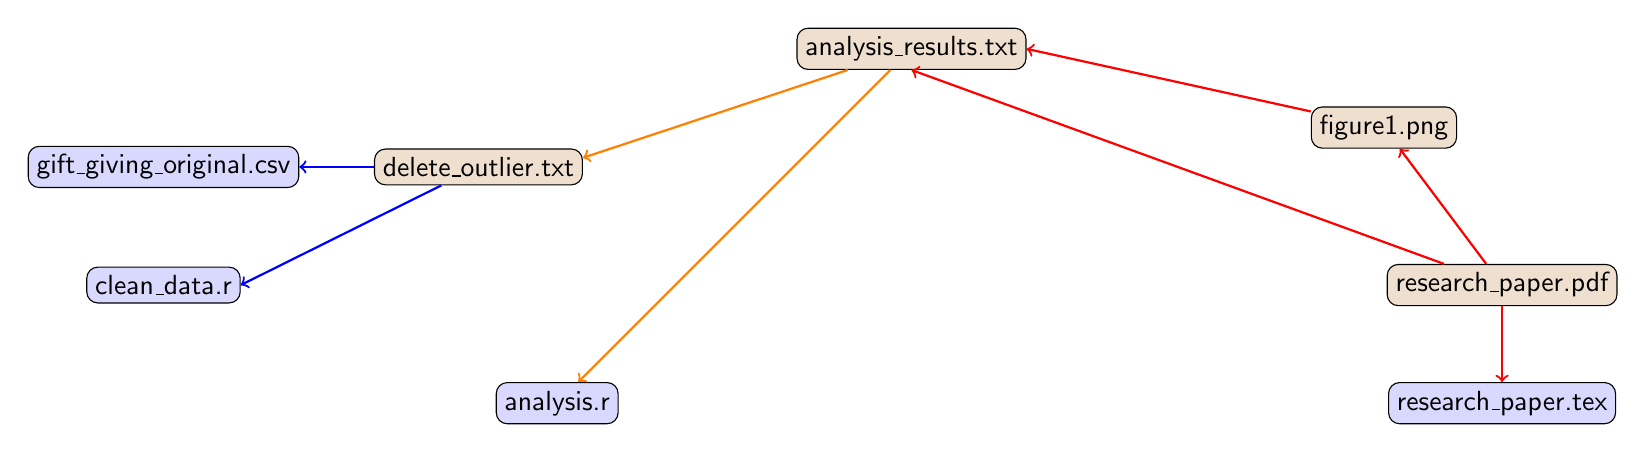
\begin{tikzpicture}[every node/.style={
    rectangle,
    rounded corners,
    inner sep=3pt,
    draw,
    fill=brown!25
}]
    \node (gift_giving_original_csv) [fill=blue!15, shift={(-6, 2)}]
    {
        gift\_giving\_original.csv
    };
    \node (clean_data_r) [fill=blue!15, shift={(-6, 0.5)}]
    {
        clean\_data.r
    };
    \node (delete_outlier_txt) [shift={(-2, 2)}]
    {
        delete\_outlier.txt
    };
    \node (analysis_r) [fill=blue!15, shift={(-1, -1)}]
    {
        analysis.r
    };


    \node (analysis_results_txt) [shift={(3.5, 3.5)}]
    {
        analysis\_results.txt
    };


      \node (research_paper_tex) [fill=blue!15, shift={(11, -1)}]
    {
        research\_paper.tex
    };
    \node (research_paper_pdf) [shift={(11, 0.5)}]
    {
        research\_paper.pdf
    };
    
    \node (figure1_png) [shift={(9.5, 2.5)}]
    {
        figure1.png
    };

    \draw[->, blue, thick] (delete_outlier_txt) to (clean_data_r.east);
    \draw[->, blue, thick] (delete_outlier_txt) to (gift_giving_original_csv);


    \draw[->, orange, thick] (analysis_results_txt) to (analysis_r);
    \draw[->, orange, thick] (analysis_results_txt) to (delete_outlier_txt.5);
    
    \draw[->, red, thick] (figure1_png) to (analysis_results_txt.east);
    
    \draw[->, red, thick] (research_paper_pdf) to (research_paper_tex.north);
    \draw[->, red, thick] (research_paper_pdf) to (figure1_png);
    \draw[->, red, thick] (research_paper_pdf) to (analysis_results_txt.south);
\end{tikzpicture}

\end{document}
